\ifdefined\includetikz\relax \else
%\documentclass{standalone}
\documentclass{article}
\usepackage{tikz}
\usepackage{amsmath}
\begin{document}
\fi

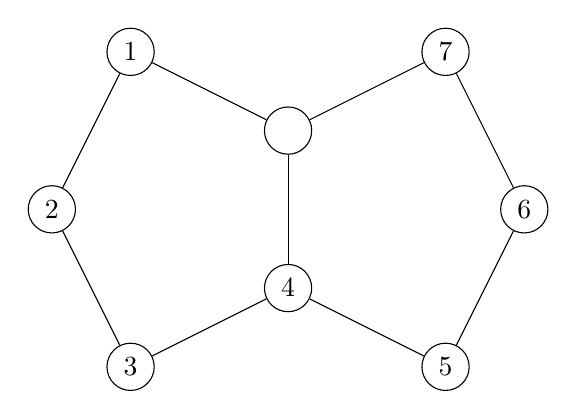
\begin{tikzpicture}[scale=1,
  piece/.style={circle, draw, inner sep= 0pt, minimum size = .6cm}
  ]
  %\def\r{.4}
  \foreach \i/\x/\y in {1/-2/3, 2/-3/1, 3/-2/-1, 4/0/0, 5/2/-1, 6/3/1, 7/2/3} {
    \node[piece] at (\x, \y) (n\i) {\i};
  }
  \node[piece] at (0, 2) (n0) {};
  \draw (n0) -- (n1) -- (n2) -- (n3) -- (n4) -- (n5) -- (n6) -- (n7) -- (n0);
  \draw (n0) -- (n4);
\end{tikzpicture}

\ifdefined\includetikz\relax \else
\end{document}
\fi
